\documentclass{article}
\usepackage[dutch]{babel}
\usepackage{hyperref}
\usepackage{graphicx}
\usepackage[bottom=2.5cm, right=2.5cm, left=2.5cm, top=2.5cm]{geometry}

\title{Startvergadering ML sessie 6}
\author{Team $\exists$uler\\
	\textit{Daan, Marie, Zeineb, Florian, Vincent, Jasper, Lasha, Younes}}
\date{Vrijdag 17 november 2023}

\begin{document}
	
	\maketitle
	
	\section*{Stand van zaken}
	
	Afgelopen week werden alle simulaties en procedures van vorige sessie afgewerkt. In figuur \ref{fig:kanban} is de status van het tabblad \textit{Implementatie} te zien vóór de aanvang van deze 6e sessie.
	
	\section*{Planning voor deze sessie}
	
	\subsection*{Bespreken van de simulaties en procedures}
	
	Deze sessie zullen we de simulaties en procedures van vorige sessie eerst en vooral met elkaar bespreken, zodat iedereen zeker op de hoogte is van wat er precies allemaal in de Python-files en Jupyter-notebooks staat. Het is belangrijk dat iedereen de geschreven code snapt. Op die manier kunnen we allemaal samen een coherent eindverslag maken en heeft iedereen genoeg kennis om tijdens de postersessie een woordje uitleg te kunnen geven.
	
	\subsection*{Uitwerken van de extra toepassing}
	
	Na het bespreken van de simulaties uit vorige sessie, zullen we de extra toepassing uitwerken.
	\\
	...
	
	\begin{figure}
		\centering
		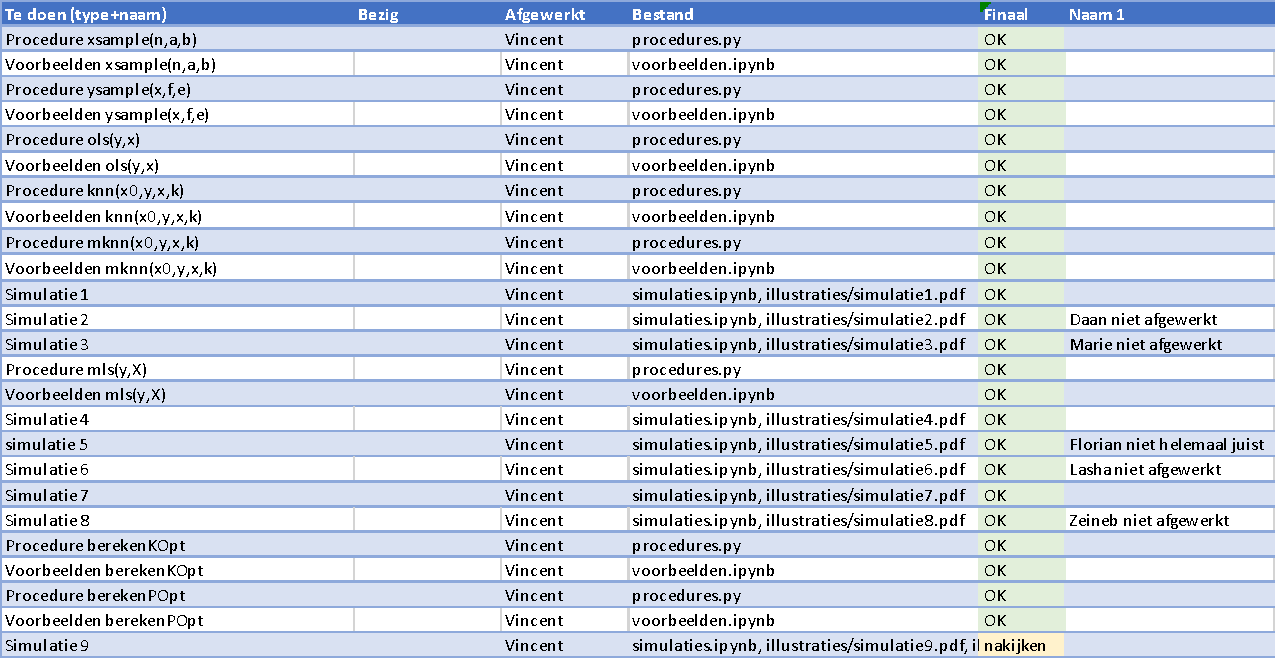
\includegraphics[width=1\textwidth]{kanban}
		\caption{De status van het tabblad \textit{Implementatie} in de KanBan vóór de aanvang van sessie 6.}
		\label{fig:kanban}
	\end{figure}
	
\end{document}